
\section{Marco Te\'orico}
\label{sec:marcoteorico}

\subsection{Tecnolog\'ias en redes fot\'onicas}
\label{sec:redfotonica}

\subsubsection{Fibra de tipo G.652.D}

Como ya se ha dicho en secciones previas, la fibra oscura a disposición es del tipo G.652.D, cuyas carácteristicas ópticas se muestran en la siguiente tabla: 

\begin{figure}[H]
  \centering
  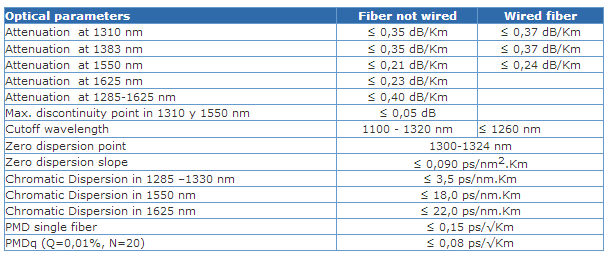
\includegraphics[scale=1]{Imagenes/Fibra.png}
  \caption{Carácteristicas ópticas fibra G.D652.D \url{http://www.telnet-ri.es/fileadmin/user_upload/hojas_producto_EN/CABLES_FO/Fibra_SM_G.652.D_EN_V1.0.pdf}}
  \label{fig:dwdmchannels}
\end{figure}

Los parámetros geométricos y mecánicos no se incluyen a fin de no saturar el presente informe, pero pueden ser encontrados en los anexos.
  
Por otro lado, sabido es el hecho de que las fibras ópticas son muy susceptibles a los factores medioambientaes, siendo dentro de los más escenciales la penetración de agua, vibración, cambios de temperatura y ataques biológicos (roedores por ejm.) o también cargas de viento y hielos para tendidos aéreos. 

\subsubsection{DWDM}
\label{sec:dwdm}

Las redes de fibra óptica modernas utilizan una tecnología de
transporte de alta capacidad llamada \emph{Dense Wavelength Division
  Multiplexing} (en español Multiplexación densa de longitud de onda),
o más comúnmente denominado por sus siglas en inglés \emph{DWDM}. Esta
tecnología permite que se puedan introducir varias señales a una misma
fibra óptica mono modo, haciendo que la transmisión goce de mayor
flexibilidad e interoperabilidad con dispositivos con inteligencia.

\emph{DWDM} opera en la capa de red, por lo que es independiente de
los protocolos de transporte y enlace. La multiplexación ocurre sobre
la banda C, es decir, a partir de la longitud de onda 1529,16 nm y
hasta 1560,61 nm. En frecuencias, esto corresponde al rango entre
192100 GHz y 196000 GHz (frecuencia central: 1931000 GHz).

A medida que aumentan los avances tecnológicos, los módulos que
trabajan con esta técnica de multiplexación incorporan mayor capacidad
al juntar cada vez más los canales en el espacio de frecuencia,
aumentando la cantidad de señales en una sola fibra. En la actualidad,
la mayor parte de las empresas de telecomunicaciones realiza diseños
que consideran espaciamientos de 100 o 50 GHz, lo que permite utilizar
la fibra con 40 ú 80 canales (o $\lambda$'s) respectivamente. No
obstante, la ciencia ya experimenta con canales espaciados por 25 e
incluso 12,5 GHz solamente, pudiendo llegarse a incorporar en el
futuro hasta 320 $\lambda$ en una sola fibra. En la jerga de
telecomunicaciones ópticas, a los distintos $\lambda$ se les llama
también ``colores'', por la similitud de conceptos en la óptica
tradicional.

\begin{figure}[H]
  \centering
  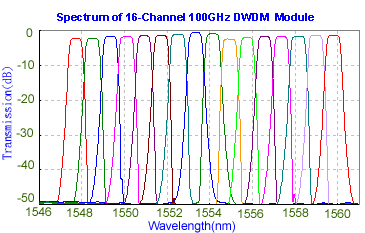
\includegraphics[scale=1]{Imagenes/DWDM_channels.png}
  \caption{Representación en el espacio frecuencial de distintas
    señales multiplexadas sobre la banda C utilizando DWDM. Se
    observan 16 canales de los 40 disponibles con un espaciamiento de
    100 GHz. Imagen obtenida del sitio
    http://sx-de-tx.wikispaces.com/DWDM+y+CWDM.}
  \label{fig:dwdmchannels}
\end{figure}

% Referencia 1: "Tecnología DWDM", G. Chavarría, C. Ramírez, 2010, Universidad de Santiago de Chile
% Referencia 2: "Tecnología DWDM", S. Bunel, 2014, Universidad de Chile

\subsubsection{OADM}
\label{sec:oadm}

Los dispositivos que se encargan de agregar o quitar $\lambda$'s de
una fibra con el fin de controlar el enlace por donde se encausan las
señales a enviar se llaman \emph{OADM}, siglas de ``optical add-drop
multiplexer''.

Existen dos tipos de \emph{OADM}. El más primitivo es el \emph{FOADM},
con la F de ``fixed'', es decir, fijo o estático. Este tipo de
direccionamiento no es reconfigurable, es decir, el diseño de la red
debe incluir los dispositivos que harán el encausamiento en los nodos
requeridos. Los filtros o LASER debían ser fijados en los nodos,
acorde a las necesidades de la red al momento de su diseño. En el caso
de requerir un cambio en la red se debían cambiar y reconectar jumpers
físicos, debiendo detener el funcionamineto de la red por el tiempo
que este proceso demorase. Además, la granularidad o precisión del
encausamiento era de a lo menos $2\lambda$, lo cual introducía
ineficiencia de recursos en la red, disminuyendo el ancho de banda de
la red a la mitad.

Debido a este inconveniente, se creó y rápidamente se reemplazó al
\emph{FOADM} por el \emph{ROADM}, con la R de
``reconfigurable''. Estos dispositivos son programables remotamente, e
incluso la conmutación puede cambiar de acuerdo a la demanda de forma
dinámica. Su granularidad es de tan solo $1\lambda$, convirtiéndose en
una opción realmente factible y adecuada para diseñar redes modernas y
flexibles.

Los dispositivos \emph{ROADM} han evolucionado desde su primera
incorporación al mercado. En un principio, los \emph{ROADM} debían
realizar demultiplexación y multiplexación de todos los canales para
poder ser flexibles, además de muchos otros inconvenientes. Esto
elevaba el costo de la red mucho pues para minimizar las pérdidas en
los nodos se debían utilizar transpondedores de calidad superior.

Los \emph{ROADM} de segunda generación mejoraban en algo los problemas
en la calidad de señal y permitían el switching de mayor calidad de
longitudes de onda individuales utilizando una técnica llama ``Wave
Blocking'' (\emph{WB}) o bloqueo de onda. El \emph{WB} solucionaba
varios de los problemas que tenían los dispositivos \emph{ROADM} de
primera generación, pero aún no eran lo suficientemente robustos,
pequeños y útiles para ser utilizados a nivel ``metro'' (redes
metropolitanas).

La tercera generación de \emph{ROADM} se llama \emph{WSS} pues
introduce la capacidad de hacer redes totalmente flexibles, de forma
dinámica y sin necesidad de tener a la cantidad de personal técnico
que se necesitaba previamente en los nodos de la red. Además, bajaron
de precio significativamente los dispositivos que ofrecían estos
servicios y aumentó con ello la oferta de dispositivos \emph{DWDM}
integrados con \emph{ROADM}.

Otra de las bondades de \emph{WSS} fue haber incorporado la
funcionalidad para interconectar redes de distintas topologías (redes
en anillo y redes en malla, por ejemplo). A estos \emph{ROADM} se les
dice que cuentan con N grados de libertad (con N la cantidad de
enlaces que conectan).

% Fuente: http://www.infonetics.com/whitepapers/infonetics-roadm-evolves-white-paper-february-2006.pdf

Las funcionalidades actuales de un \emph{ROADM} son las siguientes:
\begin{itemize}
\item \textbf{Add}: añade una señal externa a la red existente DWDM
\item \textbf{Drop}: extrae una señal de la red en el nodo donde se ejecuta la
  acción
\item \textbf{Switch}: se configura un nodo para unir dos redes y poder
  encausar el $\lambda$ a un nodo de otra red
\item \textbf{Pass-through}: se configura un nodo para no alterar a un
  $\lambda$
\end{itemize}

\subsubsection{Compensadores de atenuación}
\label{sec:amplificadores}

% Fuente: https://www.itu.int/rec/T-REC-G.663-200004-S/es

Se utilizan amplificadores ópticos para evitar la excesiva atenuación
de señal en el nodo de destino. Los amplificadores se clasifican según
su ubicación en el enlace.

El ``booster amplifier'' es un dispositivo que se inserta directamente
después del transmisor óptico. Es especialmente útil en aplicaciones
donde los \emph{OLA} o amplificadores intermedios no se pueden/quieren
insertar por algún motivo de diseño (ejemplo: redes submarinas). El
ruido que insertan es despreciable, pero una mayor potencia a su
salida repercute en distorsiones no lineales de la fibra óptica. En
ocasiones, los transmisores incluyen un ``booster amplifier''.

El preamplificador va en el receptor y sirve para mejorar la lectura
de la señal por parte del dispositivo óptico de destino. En ocasiones,
puede ir en el mismo módulo del receptor.

Los \emph{OLA} o amplificadores de línea sirven para aumentar la
potencia de forma de poder abarcar distancias de hasta miles de
kilómetros. Demasiados \emph{OLA} pueden aumentar el efecto de la
dispersión cromática no lineal y, sobre todo, aumentar los niveles de
ruido a niveles inmanejables, deteriorando demasiado el servicio de
distribución.

Todos los amplificadores pueden diseñarse de forma que el ruido que
inserten sea lo más acotado posible. Ello se logra introduciendo
filtros pasa banda adecuados a los diseños. Habiendo buenos
estándares, los filtros pueden ser diseñados de forma óptima para
casos generales.

\subsubsection{Compensadores de dispersión}
\label{sec:dispersion}

La dispersión cromática es un efecto indeseable en las redes fotónicas
multicanal como lo es, en particular, la tecnología \emph{DWDM}. La
disepersión provoca que una señal se ensanche en el dominio de la
frecuencia (o lo que es lo mismo, que se afine en el dominio del
tiempo), haciendo que sea más probable la interferencia entre
$\lambda$'s de distintos canales. Afortunadamente, este fenómeno está
ampliamente estudiado y se sabe con bastante precisión cómo reducir su
efecto a un mínimo.

Existen dos enfoques para combatir la dispersión cromática, al menos
en su componente lineal. Los enfoques son por \emph{DSP}
(procesamiento digital de señales) y por \emph{DCM} (dispersion
compensation module). El más relevante de estos enfoques por ser el
más utilizado es el \emph{DCM}, por lo que en este diseño se
utilizarán compensadores de dispersión físicos.

Todas las fibras ópticas tienen un coeficiente de dispersión cromática
que las caracteriza. El coeficiente depende de $\lambda$ y sus
unidades son $\frac{ps}{nm \times Km}$. Los \emph{DCM} son dispositivos
que se adquieren por su distancia de fibra a compensar y que tienen un
coeficiente de dispersión negativo que contrarresta el efecto de la
fibra en cuanto a la dispersión que ella intrínsecamente provoca en la
señal.

Además del efecto lineal de la dispersión, existen efectos no lineales
que se suman y se son muchísimo más complicados de compensar. Estos
son la \emph{SPM} (self phase modulation) y \emph{XPM} (cross phase
modulation). Estos efectos se producen ya que el campo eléctrico se
modula a sí mismo a medida que avanza en la fibra.

\subsection{Dispositivos presentes en una red fotónica}
\label{sec:dispositivos}

Algunos de los siguientes dispositivos expuestos en las próximas
secciones ya fueron comentados en la sección \ref{sec:redfotonica}. En
efecto, los dispositivos que aquí se presentan sirven para llevar
todos los desarrollos tecnológicos que significa la multiplexión por
\emph{DWDM} y el control de longitudes de onda por \emph{OADM} a la
práctica.

Los dispositivos que deben existir en una red óptica estándar son:
\begin{itemize}
\item \textbf{Transpondedor}: sirven para transformar una señal de
  algún protocolo de transporte típico (señales eléctricas) hacia
  longitudes de onda capaces de ser transmitidas por FO (señales
  ópticas) y vice versa.
\item \textbf{Multiplexor/demultiplexor}: los multiplexores sirven
  para seleccionar una de las longitudes de onda entrantes para
  transmitirse a la salida (concepto de multiplexación). Los
  demultiplexores hacen lo inverso; seleccionan una de las longitudes
  de onda de la entrada y la transmiten a la salida.
\item \textbf{Amplificador óptico/OLA}
\item \textbf{Canal de supervisión óptico (OSC)}: es un canal en una
  banda fuera de la banda C estándar (1510 nm nominalmente
  hablando). Sirve para transportar señales de alarma desde los
  amplificadores OLA, principalmente.
\item \textbf{DCM}: corresponde a los compensadores de dispersión
  físicos, comentados en la sección \ref{sec:dispersion}.
\end{itemize}